% CLASS 1 -- the notes' section 1.1, sec.orderDrivenMarkets.
% Budget 120 min; planned 112 over 27 frames, with the welcome frames ahead of them.
% Overrunning, cut in this order: the elementary stream (recoverable in class 2), then the
% two worked examples that do not walk the book -- the resting one and the cancellation,
% both of which the first notebook runs -- then the Sto18mic beat on the micro-price.
%
% THE FRAME CONTRACT. These slides are projection material, not reference material: the
% students read the notes, and they only ever see a frame while it is being talked over.
% So every frame carries ONE OBJECT -- a display, a statement of at most two lines, a TikZ
% picture, a table or an algorithmic block -- and under it at most three CAPTIONS. A caption
% is a gloss (`term: noun phrase'), a fragment of subject and predicate, or a condition
% written as mathematics. It is never a sentence, never a subordinate clause, and never a
% repetition of the frame title: what the title says, the body does not say again, and what
% follows from the object is spoken. At most 12 words of prose each, 25 to a frame, hard
% cap 40. A statement states its head claim and stops; its consequence is spoken.
% What is said over the object goes in \note{}, which \documentclass[script]{unito26slides}
% prints on its own and the deck itself never shows. Check with
%   python3 .claude/skills/writing-in-tex/scripts/frame_density.py <file>
%
% ORDER. The notes put prop.lobUpdate before prop.decompositionOfLimitOrder, because their
% proof of the second uses N_s, N_p and q^i from the first. The deck skips both proofs, so
% that dependency does not exist here, and the decomposition comes first: it is the one fact
% that organises the index arithmetic that follows.
%
% LABELS. The five class files are \include'd into ONE document, so a label may be defined
% once across all five, and a cross-file \ref prints ?? on a clean tree. Every statement a
% later class needs is restated there without a label. These are class 1's labels:
% lemma.orderingOfOrders, def.orderQueue, remark.sizeVersusVolume, eq.orderingOfLimitOrders,
% eq.queueImbalance, eq.microPrice, eq.fillAtLevel, eq.sweepCost,
% prop.decompositionOfLimitOrder, prop.lobUpdate, eq.elementaryStream,
% eq.transactedVolume, eq.tradedValue.
% The update display and the VWAP definition are unnumbered here, so eq.lobUpdateSellOrder
% and eq.vwap are NOT defined in this deck -- do not \ref them from a later class.
%
% A frame holds 218pt of body -- eighteen 12pt lines, or seven two-line paragraphs.

\subsection{Order-driven markets}

\begin{frame}
  \frametitle{Outline}
% One \nocite per line -- a multi-key \nocite spanning lines breaks bibtex.
\nocite{FPR13mar}
\nocite{GPWMFH13lim}
\nocite{Bou18tra}
\begin{center}
\begin{tikzpicture}[font=\scriptsize, node distance=3mm,
    stage/.style={draw=gray!60, rounded corners=2pt, align=center, inner sep=4pt,
                 text width=2.1cm, fill=gray!8},
    current/.style={stage, fill=blue!15, draw=blue!55},
    target/.style={stage, fill=orange!20, draw=orange!70}]
  \node[current] (a) {1.1\\the book};
  \node[stage, right=of a] (b) {1.2\\the fold};
  \node[stage, right=of b] (c) {1.3\\point processes};
  \node[target, right=of c] (d) {1.4\\price formation};
  \draw[-{Stealth}, gray!60] (a) -- (b);
  \draw[-{Stealth}, gray!60] (b) -- (c);
  \draw[-{Stealth}, gray!60] (c) -- (d);
\end{tikzpicture}
\end{center}

\note{
Order-driven markets are trading venues organised around limit orders: the participants
supply the prices themselves, and the venue only matches them against one another.
Two features of the data these venues produce shape everything that follows --- the events
are recorded in continuous physical time, and the occurrence of one type of event bears on
the timing of the others.
Section 1.4 asks how a price emerges from the flow of orders, and which statistics of that
flow forecast the mid-price. Everything in this class is the mechanism that question is
asked about.
}
\end{frame}

\begin{frame}
  \frametitle{Two market infrastructures}
\begin{center}
\begin{tabular}{@{}lll@{}}
\toprule
 & \emph{dealer} & \emph{limit order} \\
 & quote-driven & order-driven \\
\midrule
prices from & the dealer & the participants \\
the venue & quotes & matches \\
you observe & the dealer's quotes & every commitment, live \\
\midrule
venues & --- & Euronext, Swiss, Tokyo, \\
 & & Hong Kong, Toronto \\
 & & NYSE, NASDAQ, LSE \\
 & & (the last three keep legacy quotes) \\
\bottomrule
\end{tabular}
\end{center}

\pause

Third row: a high-frequency record of every commitment.
\note{
Market infrastructures fall in two categories. An order-driven market is transparent: every
participant observes in real time all the others' commitments to trade, organised in the
limit order book. That transparency is what makes the data exist at all, and the whole
chapter is about what can be read off it.
}
\end{frame}

\begin{frame}
  \frametitle{A limit order is four numbers}
\[
(t,q,p,d), \qquad d = +1 \text{ (buy)}, \quad d = -1 \text{ (sell)},
\qquad p \in \tickSizeOfLOB \mathbb{Z} .
\]

\pause

$p$: the \emph{worst} price accepted --- highest to buy, lowest to sell.

\pause

\emph{Cancelling}: withdrawing the commitment.
\note{
A limit order is the fundamental action a participant can perform: $t$ the time of
submission, $q$ the size in shares, $p$ the price, $d$ the direction. A participant who
posts $(t,q,p,d)$ commits at time $t$ to buy or to sell the amount $q$ at the price $p$.
By regulation $p$ is an integer multiple of a fixed tick size $\tickSizeOfLOB > 0$.
}
\end{frame}

\begin{frame}
  \frametitle{A trading epoch is the graph of a function}
\emph{trading epoch} $\tradingEpoch$: the graph of a function from $\mathbb{R}_+$ into
\[
\lbrace (q,p,d) : \, q \geq 0, \; p \geq 0, \; d = \pm 1 \rbrace .
\]

\pause

A function: no two orders share a timestamp.
\note{
A trading epoch is the collection of all limit orders submitted within a time interval.
Orders cannot be submitted simultaneously, which we say by asking that $\tradingEpoch$ be
the graph of a function: no two orders share a time. Uniqueness of timestamps is exactly
the hypothesis connexity needs on the next frame.
}
\end{frame}

\begin{frame}
  \frametitle{A match trades at the resting price}
\emph{matches}: $(s,\rho,\pi,-d)$ active, $\pi d \leq p d$. Replaced by
\[
(s,\rho - \rho \wedge q, \pi, -d),
\qquad
(t,q - \rho \wedge q, p, d).
\]

\pause

$\rho \wedge q$ shares at $\pi$ --- never at $p$.
\note{
The matching algorithm searches the active orders with timestamp $s<t$ and opposite
direction $-d$. The two orders are replaced by the pair above: $\rho \wedge q$ shares
transact, at the resting price. The single expression $\pi d \leq p d$ handles both sides: for a buy it
reads $\pi \leq p$ and for a sell $\pi \geq p$. Every fill prices at the resting order's
price, which is the fact the sweep cost and the VWAP are both built on later.
}
\end{frame}

\begin{frame}
  \frametitle{Better price first, then earlier timestamp}
\begin{equation}
\label{eq.orderingOfLimitOrders}
 (s,\rho,\pi,d) \prec (s',\rho',\pi',d)
 \quad \Longleftrightarrow \quad
 d\pi < d\pi' , \; \text{ or } \; \pi = \pi' \text{ and } s < s' .
\end{equation}

\pause

\begin{lemma}
\label{lemma.orderingOfOrders}
 The ordering \eqref{eq.orderingOfLimitOrders} is total on each side of a trading epoch.
\end{lemma}

\pause

\begin{defi}
\label{def.orderQueue}
 $\askOrderQueue_t := \lbrace (s,q,p,-1) \in \tradingEpoch : \text{active at } t \rbrace$,
 and $\bidOrderQueue_t$ with $d=+1$.
\end{defi}
\note{
Price-time priority: better price first, and at equal price the earlier timestamp.
Antisymmetry and transitivity are those of the lexicographic order on $(d\pi,s)$.
Connexity is where the epoch enters --- two distinct orders of the same side at one price
must differ in timestamp, and that is exactly what the previous frame bought.
}
\end{frame}

\begin{frame}
  \frametitle{The book is a grid of prices}
\begin{center}
\begin{tikzpicture}[x=1.05cm, y=0.0125cm, font=\scriptsize]
  \booksizeaxis{0.3}{9.2}{250}{50}
  \draw[gray!55] (0.3,0) -- (9.2,0);
  % bid side
  \foreach \x/\h in {1/150, 2/200, 3/100}
    \draw[fill=blue!55, draw=blue!70] (\x-0.24,0) rectangle (\x+0.24,\h);
  % ask side: grid position 2 is unoccupied
  \foreach \x/\h in {5/120, 7/180, 8/220}
    \draw[fill=orange!75, draw=orange!85] (\x-0.24,0) rectangle (\x+0.24,\h);
  \node[below] at (1,-4) {$\nthBestBidPrice[3]$};
  \node[below] at (2,-4) {$\nthBestBidPrice[2]$};
  \node[below] at (3,-4) {$\bestBidPrice$};
  \node[below] at (5,-4) {$\bestAskPrice$};
  \node[below] at (6,-4) {$\nthBestAskPrice[2]$};
  \node[below] at (7,-4) {$\nthBestAskPrice[3]$};
  \node[below] at (8,-4) {$\nthBestAskPrice[4]$};
  \draw[<->, gray] (1,-78) -- node[below, inner sep=1pt] {$\tickSizeOfLOB$} (2,-78);
  \draw[<->, gray] (3,250) -- node[above, fill=white, inner sep=1pt] {$\LOBspread_t$} (5,250);
  \node[orange!85!black, align=center] at (6,95) {no size\\rests here};
  \node[blue!70!black] at (1.9,235) {bid};
  \node[orange!85!black] at (7.6,258) {ask};
\end{tikzpicture}
\end{center}

\pause

Level $i$ is a \emph{position on the grid}, occupied or not.
\note{
Prices increase to the right, spaced $\tickSizeOfLOB$ apart, buy offers on the left and sell
offers on the right. The two never overlap: a buy order at or above a resting sell order
would have been matched on arrival.
The second ask level here carries nothing and is still the second ask level. Hold on to
that --- it is the distinction section 1.2 is paid for, and the sweep cost two frames from
now charges a tick for it.
}
\end{frame}

\begin{frame}
  \frametitle{Four quantities fix the book}
\[
\nthBestAskSize[i]_t
 = \sum_{\lbrace (s,q,\nthBestAskPrice[i]_t,-1) \in \askOrderQueue_t \, : \, s \leq t\rbrace} q,
\qquad
\nthBestAskPrice[i]_t = \bestAskPrice_t + (i-1)\tickSizeOfLOB ,
\]
\[
\Big( \bestAskPrice_t, \; \bestBidPrice_t, \;
\lbrace (\nthBestAskSize[i]_t, \nthBestBidSize[i]_t) : i = 1,2,\dots \rbrace \Big).
\]

\pause

In our course, a limit order book always means this \emph{aggregated} book.

\pause

No route back from a size to the orders under it.
\note{
The best ask price is the lowest at which sell offers are active, the best bid the highest
at which buy offers are, and the sizes are the sums over the queues at each level. The bid
side is symmetric, with $\nthBestBidPrice[i]_t = \bestBidPrice_t - (i-1)\tickSizeOfLOB$.
The second display is the whole state. Proposition \ref{prop.lobUpdate} is written entirely
in terms of it, which is what makes it enough.
}
\end{frame}

\begin{frame}
  \frametitle{Size is not volume}
\begin{remark}
\label{remark.sizeVersusVolume}
 \emph{Size}: the quantity queuing at a price level.\\
 \emph{Volume}: the shares transacted over an interval.
\end{remark}

\pause

Volume is not a change in size.
\note{
A level has a size at every instant; volume accumulates between two instants. So no
sequence of sizes determines the volume traded --- the same book can be reached by a trade
and by a cancellation.
What volume is, rather than what it is not: by the decomposition two frames hence,
$\volume_{t,w}$ is the sum of $\marketOrderSize$ over the market orders of the window. It is
read off the tape, and sections 1.2 and 1.4 both turn on that.
}
\end{frame}

\begin{frame}
  \frametitle{The spread is at least one tick}
\begin{defi}
 $\LOBspread_t = \abs{\bestAskPrice_t - \bestBidPrice_t}$ is the \emph{spread};
 $\midPrice_t = (\bestAskPrice_t + \bestBidPrice_t)/2$ the \emph{mid-price}.
\end{defi}

\pause

\[
\LOBspread_t \geq \tickSizeOfLOB
\qquad\text{whenever both sides are non-empty.}
\]

\pause

$\midPrice_t$: ``fundamental'' price? The reference for mark-to-market.
\note{
The two sides never overlap and every price is a multiple of $\tickSizeOfLOB$, so the
spread is at least one tick. It is not a modelling assumption: it follows from the matching
rule, so a crossed book is a bug rather than a market state.
Notice that the mid-price need not lie on the grid. On an odd spread it sits on a half tick,
and it is a derived quantity rather than a price at which anything can rest.
}
\end{frame}

\begin{frame}
  \frametitle{Imbalance is bid minus ask over the total}
\begin{defi}
 \begin{equation}
 \label{eq.queueImbalance}
 \queueImbalance[n]_t =
 \frac{\sum_{i\leq n}\nthBestBidSize[i]_t - \sum_{i\leq n}\nthBestAskSize[i]_t}
      {\sum_{i\leq n}\nthBestBidSize[i]_t + \sum_{i\leq n}\nthBestAskSize[i]_t}
 \; \in [-1,1].
 \end{equation}
\end{defi}

\pause

Bid-heavy is positive.

\pause

$i$ runs over the \emph{grid}, not over the occupied prices.
\note{
The $n$-levels queue imbalance is the normalised excess of the first $n$ bid levels over the
first $n$ ask levels.
The index runs over the grid, as on the picture three frames ago, and not over the prices
that happen to carry size. On a book with a hole the two readings differ, and section 1.2 is
where that difference is paid for --- a feed reports occupied prices, so a column slice of a
file is a different statistic that also lies in $[-1,1]$.
}
\end{frame}

\begin{frame}
  \frametitle{The micro-price weights each price by the opposite size}
\begin{defi}
 \begin{equation}
 \label{eq.microPrice}
  \microPrice_t = \midPrice_t + \frac{\LOBspread_t}{2}\queueImbalance[1]_t
  = \frac{ \nthBestBidSize[1]_t\bestAskPrice_t
         + \nthBestAskSize[1]_t\bestBidPrice_t }
         { \nthBestBidSize[1]_t + \nthBestAskSize[1]_t } .
 \end{equation}
\end{defi}

\pause

$\microPrice_t \in [\bestBidPrice_t, \bestAskPrice_t]$; bid-heavy carries it to the ask.
\note{
The second expression is an independent route to the same number, and the notebook computes
it both ways.
The name is also given to a different object, the martingale-adjusted limit of the mid-price
conditional on the imbalance \citep{Sto18mic}. The two are not the same, and the literature
does not always keep them apart --- so when a paper says micro-price, check which it means.
}
\end{frame}

\begin{frame}
  \frametitle{The sweep cost}
\begin{equation}
\label{eq.fillAtLevel}
 q_i := \Big( \quantityToLiquidate - \sum_{j<i} q_j \Big)_{+} \wedge \nthBestAskSize[i]_t ,
 \qquad \sum_{i \geq 1} q_i = \quantityToLiquidate .
\end{equation}
\begin{equation}
\label{eq.sweepCost}
 \sweepCost_t(\quantityToLiquidate)
 = \frac{1}{\quantityToLiquidate}\sum_{i\geq1} q_i
   \big(\nthBestAskPrice[i]_t - \midPrice_t\big)
 = \underbrace{\frac{\LOBspread_t}{2}}_{\text{every share}}
   + \underbrace{\frac{1}{\quantityToLiquidate}\sum_{i\geq1} q_i (i - 1)\tickSizeOfLOB}
     _{\text{its own distance, in ticks of the \emph{grid}}}
\end{equation}

\pause

Fewer than $\quantityToLiquidate$ shares on the side: undefined, so branch.
\note{
Let the ask side hold at least $\quantityToLiquidate$ shares. The first display is what the
order fills at each level, the second its per-share cost against the mid.
For a sell order the definition is the same with the bid side, and
$\midPrice_t - \nthBestBidPrice[i]_t$ in place of
$\nthBestAskPrice[i]_t - \midPrice_t$.
The second term is a grid distance and not a count of queues, which the picture two frames
on is about.
}
\end{frame}

\begin{frame}
  \frametitle{The sweep cost, visualised}
\begin{center}
\begin{tikzpicture}[x=0.72cm, y=0.0125cm, font=\tiny]
  \begin{scope}
    \booksizeaxis{0.4}{4.7}{200}{50}
    \draw[gray!55] (0.4,0) -- (4.7,0);
    \draw[fill=blue!55, draw=blue!70] (1-0.26,0) rectangle (1+0.26,100);
    \draw[fill=orange!30, draw=orange!60] (3-0.26,0) rectangle (3+0.26,120);
    \draw[fill=orange!30, draw=orange!60] (4-0.26,0) rectangle (4+0.26,180);
    \draw[fill=orange!85, draw=orange!90] (3-0.26,0) rectangle (3+0.26,120);
    \draw[fill=orange!85, draw=orange!90] (4-0.26,0) rectangle (4+0.26,130);
    \draw[dashed, gray!70] (2,0) -- (2,150);
    \node[below] at (1,-4) {$1000$}; \node[below] at (2,-4) {$1001$};
    \node[below] at (3,-4) {$1002$}; \node[below] at (4,-4) {$1003$};
    \node[gray!50!black, above, inner sep=1pt] at (2,150) {$\midPrice_{t-}$};
    \node[white] at (3,60) {$120$}; \node[white] at (4,65) {$130$};
    \node at (3.6,225) {before};
  \end{scope}
  \draw[-{Stealth}, gray!55] (5.0,120) -- node[above, inner sep=2pt, text=black]
       {buy $250$ at $1003$} (7.8,120);
  \begin{scope}[xshift=5.9cm]
    \booksizeaxis{0.4}{4.7}{200}{50}
    \draw[gray!55] (0.4,0) -- (4.7,0);
    \draw[fill=blue!55, draw=blue!70] (1-0.26,0) rectangle (1+0.26,100);
    \draw[fill=orange!75, draw=orange!85] (4-0.26,0) rectangle (4+0.26,50);
    \node[below] at (1,-4) {$1000$}; \node[below] at (2,-4) {$1001$};
    \node[below] at (3,-4) {$1002$}; \node[below] at (4,-4) {$1003$};
    \node at (3.6,225) {after};
  \end{scope}
\end{tikzpicture}
\end{center}

\pause

\[
 \sweepCost_t(250)
 = \frac{120 \cdot 1 + 130 \cdot 2}{250} \, \tickSizeOfLOB
 = \underbrace{1}_{\LOBspread_t / 2} + \underbrace{0.52}_{\text{the walk}}
   \quad \text{ticks} .
\]

\pause

One tick of spread; $130$ shares one tick further.
\note{
The book is the one the worked examples run on: best bid $1000$ for $100$, ask $1002$ for
$120$ and $1003$ for $180$, so the mid is $1001$ and the spread two ticks.
The order takes $120$ at $1002$ and $130$ at $1003$, and $50$ shares are left resting at
$1003$: the best ask moves up a tick and the spread widens to three.
Every one of the $250$ shares pays the half-spread; only the $130$ that reach the second
occupied level pay the extra tick, and they pay it because of where that level sits on the
\emph{grid}, not because it is the second queue.
}
\end{frame}

\begin{frame}
  \frametitle{An empty level still charges its tick}
\begin{center}
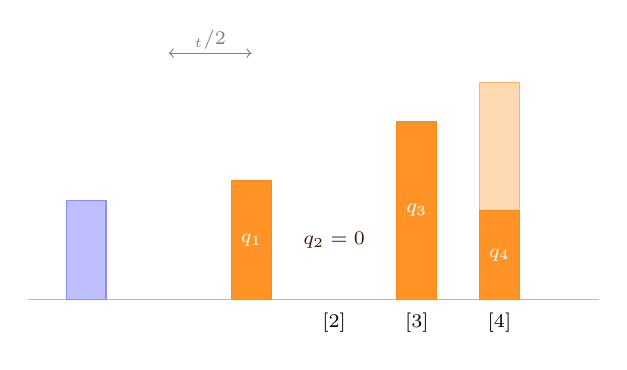
\begin{tikzpicture}[x=1.05cm, y=0.0125cm, font=\scriptsize]
  \booksizeaxis{2.3}{9.2}{250}{50}
  \draw[gray!55] (2.3,0) -- (9.2,0);
  \draw[fill=blue!25, draw=blue!45] (3-0.24,0) rectangle (3+0.24,100);
  \draw[fill=orange!30, draw=orange!60] (5-0.24,0) rectangle (5+0.24,120);
  \draw[fill=orange!30, draw=orange!60] (7-0.24,0) rectangle (7+0.24,180);
  \draw[fill=orange!30, draw=orange!60] (8-0.24,0) rectangle (8+0.24,220);
  \draw[fill=orange!85, draw=orange!90] (5-0.24,0) rectangle (5+0.24,120);
  \draw[fill=orange!85, draw=orange!90] (7-0.24,0) rectangle (7+0.24,180);
  \draw[fill=orange!85, draw=orange!90] (8-0.24,0) rectangle (8+0.24,90);
  \node[below] at (3,-4) {$\bestBidPrice$};
  \node[below] at (5,-4) {$\bestAskPrice$};
  \node[below] at (6,-4) {$\nthBestAskPrice[2]$};
  \node[below] at (7,-4) {$\nthBestAskPrice[3]$};
  \node[below] at (8,-4) {$\nthBestAskPrice[4]$};
  \node[white] at (5,60) {$q_1$};
  \node[orange!20!black] at (6,60) {$q_2=0$};
  \node[white] at (7,90) {$q_3$};
  \node[white] at (8,45) {$q_4$};
  \draw[<->, gray] (4,250) -- node[above, fill=white, inner sep=1pt] {$\LOBspread_t/2$} (5,250);
\end{tikzpicture}
\end{center}

\pause

Shaded: what a buy order for $\quantityToLiquidate$ shares takes.

\pause

The third level pays two ticks, not one.
\note{
The second ask level is empty, so $q_2 = 0$, and the third one is two ticks from the touch
whether or not anything rests between them. The distance the sweep cost charges is a grid
distance and not a count of queues, which is the whole reason the previous display is
written with $(i-1)\tickSizeOfLOB$ rather than with a running index over occupied prices.
}
\end{frame}

\begin{frame}
  \frametitle{Every limit order is a market order and a resting order}
\begin{prop}
\label{prop.decompositionOfLimitOrder}
 Processing $(t,q,p,-1)$ against the book at $t-$ is processing the ordered pair
 \[
 \big[\,(t,\marketOrderSize,0,-1)\,,\;(t,q-\marketOrderSize,p,-1)\,\big],
 \]
 \[
 \marketOrderSize := \min\Big(q, \; \textstyle\sum_{i\geq 1} \nthBestBidSize[i]_{t-}
 \indicator{\nthBestBidPrice[i]_{t-}\geq p}\Big),
 \]
 the first having priority. For a buy, $\infty$ in place of $0$ and the ask side under
 $\nthBestAskPrice[i]_{t-} \leq p$.
\end{prop}

\pause

One code path: consume, then rest the remainder.
\note{
The first component is the market order: the price $0$ for a sell, $\infty$ for a buy, is a
price \emph{specification} guaranteeing immediate execution and not a price at which
anything may rest. The second is exactly the part that rests.
An implementation that writes a separate branch for a marketable order has two code paths
where the mathematics has one, and the two will drift.
}
\end{frame}

\begin{frame}
  \frametitle{Walking costs more than the half-spread}
\emph{walks the book}: reaches past the best level.
\[
\marketOrderSize > \nthBestBidSize[1]_{t-} \text{ (sell)},
\qquad
\marketOrderSize > \nthBestAskSize[1]_{t-} \text{ (buy)},
\qquad\Longleftrightarrow\qquad
\sweepCost_t(\quantityToLiquidate) > \frac{\LOBspread_t}{2} .
\]

\pause

The walk term of \eqref{eq.sweepCost} is positive: some $q_i > 0$, $i \geq 2$.

\pause

Walking implies $N \geq 1$ below; the converse fails.
\note{
The equivalence holds wherever the sweep cost is defined, which is where the side holds the
shares asked for.
The converse of the second claim fails because an order that clears the best level exactly
moves the best price, so $N = 1$, yet it prints at a single price and walks nothing.
Over a window, the seller-initiated trades are the components $(t,\marketOrderSize,0,-1)$
with $\marketOrderSize > 0$, and the buyer-initiated ones the components with $\infty$. We
adopt that as our convention for the word \emph{trade}, on venues that accept genuine market
orders too.
}
\end{frame}

\begin{frame}
  \frametitle{An order clears one level at a time}
\begin{equation}
\label{eq.elementaryStream}
 (t,\nthBestBidSize[1]_{t-},\nthBestBidPrice[1]_{t-},-1), \dots,
 (t,\nthBestBidSize[N]_{t-},\nthBestBidPrice[N]_{t-},-1),
 (t,q^{N}, p, -1),
\end{equation}
with priority from left to right, $N$ the levels consumed in full.

\pause

\emph{Elementary}: clears one level, or rests without matching.

\pause

Why the fold of section 1.2 terminates.
\note{
The market part may reach any depth, and it can be decomposed one level at a time. That is
what the update rule of the next two frames is bookkeeping for.
The termination argument matters in class 2: each pass of the loop empties one price, so the
loop is finite because the book is.
}
\end{frame}

% algo.bookFold of the notes, cut to the matching loop: the message, the stream and the
% fold are class 2's objects, and the full listing stays in message_files.tex.
% `algorithm' is a float and floats do not place inside a frame, so the environment is
% bare -- no caption, no line numbering, no \label{algo.*} -- and carries no \pause.
\begin{frame}
  \frametitle{The rule is a loop before it is a formula}
{\footnotesize
\begin{algorithmic}
 \REQUIRE the book at $t-$, and the order $(t,q,p,d)$
 \STATE set the market part $\marketOrderSize$ by
        Proposition \ref{prop.decompositionOfLimitOrder}, and $r := \marketOrderSize$
 \WHILE{$r > 0$}
 \STATE let $\pi$ be the best price-eligible price on the side $-d$
 \STATE match $r$ against the size resting at $\pi$, at $\pi$
 \STATE subtract the matched shares, remove $\pi$ if it empties,
        and decrease $r$ by the same amount
 \ENDWHILE
 \STATE add $q - \marketOrderSize$ to the size at $p$ on the side $d$
\end{algorithmic}
}

\pause

The next two frames are this loop, closed.
\note{
Each pass of the loop empties one price, so the loop is finite because the book is: this is
the elementary stream of the previous frame, read as a procedure.
The two frames that follow are the same rule in closed form, which is what an implementation
is checked against rather than what it is written from.
In class 2 the procedure gains the branch for a cancellation, the state
$\mathcal{B}_{k-1}$ it carries and the value $\mathcal{B}_{k}$ it returns, and becomes the
fold of the message stream.
}
\end{frame}

\begin{frame}
  \frametitle{The update rule --- 1 of 2}
\begin{prop}
\label{prop.lobUpdate}
 Let $(t,q,p,-1)$ arrive with
 $q < \sum_{i\geq1}\nthBestBidSize[i]_{t-}\indicator{\nthBestBidPrice[i]_{t-}\geq p}$. Put
 \[
 N_s := \inf\Big\lbrace n \geq 0 : q < \textstyle\sum_{i=1}^{n}
 \nthBestBidSize[i]_{t-}\Big\rbrace,
 \qquad
 N_p := \inf\lbrace n \geq 1 : \nthBestBidPrice[n]_{t-} < p \rbrace,
 \]
 \[
 N := \max(0, \, N_s \wedge N_p - 1),
 \qquad
 q^{i} := \max\Big(0, \, q - \textstyle\sum_{1 \leq k \leq i} \nthBestBidSize[k]_{t-}
 \indicator{\nthBestBidPrice[k]_{t-} \geq p}\Big).
 \]
\end{prop}

\pause

$N_s$: size runs out. $N_p$: the price constraint bites.\\
$\inf\emptyset = +\infty$.
\note{
$N$ is the number of bid levels consumed in full, and $q^i$ the quantity still to be
executed once the first $i$ levels are gone.
Both infima may be over an empty set. $N_s$ carries no price constraint, so it is infinite
when $q$ exceeds the \emph{total} bid size --- not the price-eligible one --- and $N_p$ is
infinite for a market order, since prices are non-negative.
The hypothesis is that the order does not consume the whole price-eligible side. When it
does, the best price on that side is undefined and the rule does not apply.
}
\end{frame}

\begin{frame}
  \frametitle{The update rule --- 2 of 2}
\[
 \bestBidPrice_t = \nthBestBidPrice[1+N]_{t-},
 \qquad
 \nthBestBidSize[k]_{t} = \nthBestBidSize[k+N]_{t-} - \big( q^{k+N-1}-q^{k+N} \big),
\]
\[
 \bestAskPrice_t = \bestAskPrice_{t-} - \max(0,\bestAskPrice_{t-} - p)
 \indicator{q^{\infty} > 0},
\]
\[
 \nthBestAskSize[k]_t = \nthBestAskSize[k+\delta\bestAskPrice_t/\tickSizeOfLOB]_{t-}
 + q^{\infty}\indicator{p=\bestAskPrice_t + (k-1)\tickSizeOfLOB} ,
\]
\[
\delta\bestAskPrice_t := \bestAskPrice_t - \bestAskPrice_{t-} \leq 0,
\qquad
\nthBestAskSize[j]_{t-} = \nthBestBidSize[j]_{t-} = 0 \; \text{ for } j \leq 0 .
\]

\pause

Bid: shifts up by $N$. Ask: untouched unless a residual rests.
\note{
Reading the four lines: the bid side shifts up by the $N$ levels consumed, and the new best
bid may be partially eaten; the ask side is untouched unless something is left over.
If $q^{\infty} > 0$ the residual rests at $p$, improving the best ask when
$p < \bestAskPrice_{t-}$ and shifting every ask index by
$-\delta\bestAskPrice_t/\tickSizeOfLOB$ levels.
For a buy order the rules are the same with the sides interchanged. The next frame is the
picture.
}
\end{frame}

\begin{frame}
  \frametitle{A resting order can improve the best price}
\begin{center}
\begin{tikzpicture}[x=0.54cm, y=0.0125cm, font=\tiny]
  \begin{scope}
    \booksizeaxis{0.4}{6.6}{200}{50}
    \draw[gray!55] (0.4,0) -- (6.6,0);
    \draw[fill=blue!55, draw=blue!70] (1-0.26,0) rectangle (1+0.26,150);
    \draw[fill=blue!55, draw=blue!70] (2-0.26,0) rectangle (2+0.26,200);
    \draw[fill=blue!55, draw=blue!70] (3-0.26,0) rectangle (3+0.26,100);
    \draw[fill=orange!75, draw=orange!85] (5-0.26,0) rectangle (5+0.26,120);
    \draw[fill=orange!75, draw=orange!85] (6-0.26,0) rectangle (6+0.26,180);
    \node[below] at (1,-4) {$998$}; \node[below] at (2,-4) {$999$};
    \node[below] at (3,-4) {$1000$}; \node[below] at (4,-4) {$1001$};
    \node[below] at (5,-4) {$1002$}; \node[below] at (6,-4) {$1003$};
    \node at (3.5,240) {before};
  \end{scope}
  \draw[-{Stealth}, gray!55] (7.0,120) -- node[above, inner sep=2pt, text=black] {buy $50$ at $1001$} (10.3,120);
  \begin{scope}[xshift=5.9cm]
    \booksizeaxis{0.4}{6.6}{200}{50}
    \draw[gray!55] (0.4,0) -- (6.6,0);
    \draw[fill=blue!55, draw=blue!70] (1-0.26,0) rectangle (1+0.26,150);
    \draw[fill=blue!55, draw=blue!70] (2-0.26,0) rectangle (2+0.26,200);
    \draw[fill=blue!55, draw=blue!70] (3-0.26,0) rectangle (3+0.26,100);
    \draw[fill=blue!55, draw=blue!70] (4-0.26,0) rectangle (4+0.26,50);
    \draw[fill=orange!75, draw=orange!85] (5-0.26,0) rectangle (5+0.26,120);
    \draw[fill=orange!75, draw=orange!85] (6-0.26,0) rectangle (6+0.26,180);
    \node[below] at (1,-4) {$998$}; \node[below] at (2,-4) {$999$};
    \node[below] at (3,-4) {$1000$}; \node[below] at (4,-4) {$1001$};
    \node[below] at (5,-4) {$1002$}; \node[below] at (6,-4) {$1003$};
    \node at (3.5,240) {after};
  \end{scope}
\end{tikzpicture}
\end{center}

\pause

$N = 0$, $q^{\infty} = q$: nothing matches, the spread narrows to a tick.
\note{
The price $1001$ is below every resting ask, so the order matches nothing and the whole of
it rests. It rests inside the old spread, which is how a best price improves without a
single share trading.
This is the baseline the next three frames are read against: the same book each time, and
one order or one cancellation against it.
}
\end{frame}

\begin{frame}
  \frametitle{Executed in full, and nothing rests}
\begin{center}
\begin{tikzpicture}[x=0.54cm, y=0.0125cm, font=\tiny]
  \begin{scope}
    \booksizeaxis{0.4}{6.6}{200}{50}
    \draw[gray!55] (0.4,0) -- (6.6,0);
    \draw[fill=blue!55, draw=blue!70] (1-0.26,0) rectangle (1+0.26,150);
    \draw[fill=blue!55, draw=blue!70] (2-0.26,0) rectangle (2+0.26,200);
    \draw[fill=blue!55, draw=blue!70] (3-0.26,0) rectangle (3+0.26,100);
    \draw[fill=orange!75, draw=orange!85] (5-0.26,0) rectangle (5+0.26,120);
    \draw[fill=orange!75, draw=orange!85] (6-0.26,0) rectangle (6+0.26,180);
    \node[below] at (1,-4) {$998$}; \node[below] at (2,-4) {$999$};
    \node[below] at (3,-4) {$1000$}; \node[below] at (4,-4) {$1001$};
    \node[below] at (5,-4) {$1002$}; \node[below] at (6,-4) {$1003$};
    \node at (3.5,240) {before};
  \end{scope}
  \draw[-{Stealth}, gray!55] (7.0,120) -- node[above, inner sep=2pt, text=black] {sell $250$ at $999$} (10.3,120);
  \begin{scope}[xshift=5.9cm]
    \booksizeaxis{0.4}{6.6}{200}{50}
    \draw[gray!55] (0.4,0) -- (6.6,0);
    \draw[fill=blue!55, draw=blue!70] (1-0.26,0) rectangle (1+0.26,150);
    \draw[fill=blue!55, draw=blue!70] (2-0.26,0) rectangle (2+0.26,50);
    \draw[fill=orange!75, draw=orange!85] (5-0.26,0) rectangle (5+0.26,120);
    \draw[fill=orange!75, draw=orange!85] (6-0.26,0) rectangle (6+0.26,180);
    \node[below] at (1,-4) {$998$}; \node[below] at (2,-4) {$999$};
    \node[below] at (3,-4) {$1000$}; \node[below] at (4,-4) {$1001$};
    \node[below] at (5,-4) {$1002$}; \node[below] at (6,-4) {$1003$};
    \node at (3.5,240) {after};
  \end{scope}
\end{tikzpicture}
\end{center}

\pause

$N_p$ bites before $N_s$: $q^{\infty} = 0$, the ask side untouched.
\note{
The order takes $100$ at $1000$ and $150$ of the $200$ resting at $999$, which is its own
limit price. Nothing is left over, so nothing rests and the ask side does not move.
The best bid falls one level and the spread widens from two ticks to three: an execution
widens the spread by consuming a queue, never by moving a price the other way.
}
\end{frame}

\begin{frame}
  \frametitle{The residual rests below the old best bid}
\begin{center}
\begin{tikzpicture}[x=0.54cm, y=0.0125cm, font=\tiny]
  \begin{scope}
    \booksizeaxis{0.4}{6.6}{200}{50}
    \draw[gray!55] (0.4,0) -- (6.6,0);
    \foreach \x/\h in {1/150, 2/200, 3/100}
      \draw[fill=blue!55, draw=blue!70] (\x-0.26,0) rectangle (\x+0.26,\h);
    \foreach \x/\h in {5/120, 6/180}
      \draw[fill=orange!75, draw=orange!85] (\x-0.26,0) rectangle (\x+0.26,\h);
    \node[below] at (1,-4) {$998$}; \node[below] at (2,-4) {$999$};
    \node[below] at (3,-4) {$1000$}; \node[below] at (4,-4) {$1001$};
    \node[below] at (5,-4) {$1002$}; \node[below] at (6,-4) {$1003$};
    \node at (3.5,240) {before};
  \end{scope}
  \draw[-{Stealth}, gray!55] (7.0,120) -- node[above, inner sep=2pt, text=black] {sell $400$ at $999$} (10.3,120);
  \begin{scope}[xshift=5.9cm]
    \booksizeaxis{0.4}{6.6}{200}{50}
    \draw[gray!55] (0.4,0) -- (6.6,0);
    \draw[fill=blue!55, draw=blue!70] (1-0.26,0) rectangle (1+0.26,150);
    \draw[fill=orange!75, draw=orange!85] (2-0.26,0) rectangle (2+0.26,100);
    \foreach \x/\h in {5/120, 6/180}
      \draw[fill=orange!75, draw=orange!85] (\x-0.26,0) rectangle (\x+0.26,\h);
    \node[below] at (1,-4) {$998$}; \node[below] at (2,-4) {$999$};
    \node[below] at (3,-4) {$1000$}; \node[below] at (4,-4) {$1001$};
    \node[below] at (5,-4) {$1002$}; \node[below] at (6,-4) {$1003$};
    \node at (3.5,240) {after};
  \end{scope}
\end{tikzpicture}
\end{center}

\pause

$N = 2$, $q^{\infty} = 100$, and every ask index shifts by three.

\pause

Two ask levels, $1000$ and $1001$, are now empty and still counted.
\note{
The order takes $100$ at $1000$ and $200$ at $999$, so two levels are consumed in full and a
hundred shares are left over. They rest at the order's own limit price, $999$ --- on a level
it has just cleared, which is now on the ask side.
Since $999 < \bestAskPrice_{t-} = 1002$, the best ask improves by three ticks and every ask
index shifts by three. This is the case people get wrong: the residual is not inside the old
spread.
}
\end{frame}

\begin{frame}
  \frametitle{A cancellation moves the best bid down}
\begin{center}
\begin{tikzpicture}[x=0.54cm, y=0.0125cm, font=\tiny]
  \begin{scope}
    \booksizeaxis{0.4}{6.6}{200}{50}
    \draw[gray!55] (0.4,0) -- (6.6,0);
    \draw[fill=blue!55, draw=blue!70] (1-0.26,0) rectangle (1+0.26,150);
    \draw[fill=blue!55, draw=blue!70] (2-0.26,0) rectangle (2+0.26,200);
    \draw[fill=blue!55, draw=blue!70] (3-0.26,0) rectangle (3+0.26,100);
    \draw[fill=orange!75, draw=orange!85] (5-0.26,0) rectangle (5+0.26,120);
    \draw[fill=orange!75, draw=orange!85] (6-0.26,0) rectangle (6+0.26,180);
    \node[below] at (1,-4) {$998$}; \node[below] at (2,-4) {$999$};
    \node[below] at (3,-4) {$1000$}; \node[below] at (4,-4) {$1001$};
    \node[below] at (5,-4) {$1002$}; \node[below] at (6,-4) {$1003$};
    \node at (3.5,240) {before};
  \end{scope}
  \draw[-{Stealth}, gray!55] (7.0,120) -- node[above, inner sep=2pt, text=black] {withdraw $100$ at $1000$} (10.3,120);
  \begin{scope}[xshift=5.9cm]
    \booksizeaxis{0.4}{6.6}{200}{50}
    \draw[gray!55] (0.4,0) -- (6.6,0);
    \draw[fill=blue!55, draw=blue!70] (1-0.26,0) rectangle (1+0.26,150);
    \draw[fill=blue!55, draw=blue!70] (2-0.26,0) rectangle (2+0.26,200);
    \draw[fill=orange!75, draw=orange!85] (5-0.26,0) rectangle (5+0.26,120);
    \draw[fill=orange!75, draw=orange!85] (6-0.26,0) rectangle (6+0.26,180);
    \node[below] at (1,-4) {$998$}; \node[below] at (2,-4) {$999$};
    \node[below] at (3,-4) {$1000$}; \node[below] at (4,-4) {$1001$};
    \node[below] at (5,-4) {$1002$}; \node[below] at (6,-4) {$1003$};
    \node at (3.5,240) {after};
  \end{scope}
\end{tikzpicture}
\end{center}

\pause

The spread widens, and not one share traded.
\note{
The whole of the best bid queue is withdrawn, so $1000$ leaves the book and the best bid
becomes $999$. The spread widens from two ticks to three, and not one share has traded.
A size falls for two reasons and only one of them is a trade, which is the content of the
remark on size against volume, and the reason the volume over a window cannot be read off
the sequence of configurations.
}
\end{frame}

\begin{frame}
  \frametitle{Volume is a sum over market orders}
\begin{defi}
 \begin{equation}
 \label{eq.transactedVolume}
  \volume_{t,w} := \sum_{n \, : \, t-w < \arrivalTimes[]_n \leq t} \marketOrderSize[n] ,
 \end{equation}
 \begin{equation}
 \label{eq.tradedValue}
  \tradedValue_{t,w} := \sum_{n \, : \, t-w < \arrivalTimes[]_n \leq t}
  \sum_{i \geq 1} q_{n,i} \, \pi_{n,i} ,
 \end{equation}
 and $\vwap_{t,w} := \tradedValue_{t,w}/\volume_{t,w}$ where $\volume_{t,w} > 0$.
\end{defi}

\pause

Every fill in \eqref{eq.tradedValue} prices at $\pi_{n,i}$, the \emph{resting} price.
\note{
Let $(\arrivalTimes[]_n, \marketOrderSize[n], d_n)$ be the stream of market orders of a
trading epoch, and $q_{n,i}$ the fills of the $n$-th of them, at prices $\pi_{n,i}$. A market
order does not in general execute at a single price, which is why the traded value is a
double sum and not a product.
The volume-weighted average price is defined whenever anything traded in the window.
}
\end{frame}

\begin{frame}
  \frametitle{VWAP reads the tape, the sweep cost reads the book}
\begin{remark}
 $\vwap_{t,w}$ is a statistic of the \emph{transactions}.
\end{remark}

\pause

cf.\ Remark \ref{remark.sizeVersusVolume}.

\pause

The sweep cost prices an order that is never submitted.
\note{
The VWAP cannot be recovered from the sequence of configurations alone. A level shrinks by
cancellation as well as by execution, so no sequence of sizes determines the volume traded,
and therefore none determines the VWAP.
The sweep cost, by contrast, is a function of one configuration, defined whether or not the
order it prices is ever submitted. One quantity needs the tape and one needs only the book.
In class 2 that is exactly why a LOBSTER pair is read together --- the orderbook file alone
determines no volume.
Section 1.2 next: where the sequence of configurations comes from, and why a participant
computes it rather than receiving it. Section 1.4 is where all of it is going.
}
\end{frame}
